% Chapter 4. Material: docs/architecture/, docs/adr/, docs/data/, docs/security/, docs/pedagogy/,
% docs/process/agent-harness.md, src/muallim/. Figures: fig-context, fig-layers, fig-pipeline, fig-harness,
% screens 07_line.png and 09_result_errors.png (docs/design/screens/).
\chapter{Implementation}\label{ch:impl}

This chapter describes the artefacts as built in version 0.6.0. Sections~\ref{sec:impl-overview}--%
\ref{sec:impl-privacy} cover the tutor: its context, the curriculum, the architecture, the assessment
pipeline, the learner interface, the research data, the training pipeline of the adapted model
(Section~\ref{sec:impl-training}, still a design), the mastery models (Section~\ref{sec:impl-mastery}, still a
design) and privacy. Section~\ref{sec:impl-harness} describes
the development harness, and Section~\ref{sec:impl-verification} the verification of both.

\section{Overview}\label{sec:impl-overview}

Figure~\ref{fig:context} shows the system in its context. A learner talks to the tutor through the Telegram
Bot API, using buttons and voice messages. The tutor takes lessons from a curriculum built from the book,
sends the learner's audio to the Quran Muaalem recogniser, and stores attempts, errors and annotations in
PostgreSQL; audio files are kept in a separate store and only with consent. A researcher works with the data
through a command-line tool that builds reports, prepares annotation packages and exports datasets.
Annotators, two teachers, label attempts either in Telegram or in spreadsheet packages.

\begin{figure}[ht]
\centering
\resizebox{0.95\linewidth}{!}{% Контекст системы (C4, уровень 1). Источник смысла: docs/architecture/diagrams/01-context.mmd.
\begin{tikzpicture}[node distance=6mm and 9mm]
  \node[human,text width=2.6cm] (learner) {\LANG{Learner}{Ученик}\\[-1pt]{\scriptsize\LANG{Russian-speaking beginner}{русскоязычный новичок}}};
  \node[box,right=of learner,text width=2.2cm] (tg) {Telegram\\Bot API};
  \node[hot,right=of tg,text width=3.0cm] (bot) {\LANG{Tutor bot}{Бот-тренажёр}\\[-1pt]{\scriptsize Python 3.12, aiogram 3}};
  \node[box,above=of bot,text width=3.0cm] (book) {\LANG{Curriculum}{Программа}\\[-1pt]{\scriptsize\LANG{125 lessons, book order}{125 уроков в порядке книги}}};
  \node[box,right=of bot,text width=2.6cm] (model) {Quran Muaalem\\[-1pt]{\scriptsize\LANG{phoneme recogniser}{распознавание фонем}}};
  \node[store,below=of bot,text width=2.9cm,minimum height=1.1cm] (db) {PostgreSQL\\[-1pt]{\scriptsize\LANG{attempts, errors, labels}{попытки, ошибки, метки}}};
  \node[store,right=of db,text width=2.4cm,minimum height=1.1cm] (audio) {\LANG{Audio store}{Записи}\\[-1pt]{\scriptsize\LANG{consent only}{только с согласия}}};
  \node[box,left=of db,text width=2.9cm] (cli) {muallim-research\\[-1pt]{\scriptsize\LANG{reports, labels, dataset}{отчёты, разметка, датасет}}};
  \node[human,below=of cli,text width=2.6cm] (res) {\LANG{Researcher}{Исследователь}};
  \node[human,below=of db,text width=2.9cm] (ann) {\LANG{Annotators}{Разметчики}\\[-1pt]{\scriptsize\LANG{two teachers}{два преподавателя}}};

  \draw[arr] (learner) -- node[lab,below]{\LANG{voice, taps}{голос, кнопки}} (tg);
  \draw[arr] (tg) -- (bot);
  \draw[arr] (book) -- (bot);
  \draw[arr] (bot) -- (model);
  \draw[arr] (bot) -- (db);
  \draw[arr] (bot.south east) -- (audio.north west);
  \draw[arr] (res) -- (cli);
  \draw[arr] (cli) -- (db);
  \draw[arr,<->] (ann) -- node[lab,left,pos=0.3]{\LANG{labels}{метки}} (db);
  \begin{scope}[on background layer]
    \node[group,fit=(bot)(book)(db)(audio)(cli)(model),label={[lab,anchor=south east]north east:\LANG{system boundary}{граница системы}}] {};
  \end{scope}
\end{tikzpicture}
}
\caption{System context (R-01).}\label{fig:context}
\end{figure}

The code is written in Python 3.12 and has about 9\,000 lines in 92 modules. Table~\ref{tab:stack} lists
the main technologies and the reason for each choice.

\begin{table}[ht]
\centering\small
\caption{Technology stack.}
\label{tab:stack}
\begin{tabularx}{\linewidth}{@{}P{3.1cm}P{4.2cm}L@{}}
\toprule
Concern & Choice & Reason \\
\midrule
Messenger & Telegram, aiogram 3 & Audience already uses it; voice messages; asynchronous, typed library. \\
Recogniser & Quran Muaalem \cite{SRC-003} & Open, phoneme-level, with articulatory attributes. \\
Dependency injection & dishka \cite{SRC-008} & Application and request scopes; aiogram integration. \\
Database & PostgreSQL 16, SQLAlchemy Core, Alembic & Research data with migrations; SQLite in tests. \\
Architecture checks & import-linter \cite{SRC-009} & Layer contracts enforced in CI and by the agent's
stop hook. \\
Quality & pytest, Hypothesis, mypy --strict, ruff & Fast tests without model or network; strict types. \\
Packaging & uv, Docker & Lock file; reproducible image; model as an optional extra. \\
\bottomrule
\end{tabularx}
\end{table}

\section{Curriculum from the book}\label{sec:impl-curriculum}

\paragraph{Edition and transcription} The 2010 Almetyevsk edition \cite{SRC-040} was chosen because it is a
complete modern edition issued by a Muslim board, follows the orthography of the Medina mushaf --- the same
orthography as the model's data --- and its letter order agrees with an independent Uzbek edition, which
indicates that the order is Maksudi's own. The exercise pages 10--85 were transcribed line by line. The
scan of the book is kept locally and outside version control and the bot: the edition is copyrighted, so
the tutor contains only the Arabic exercises and its own explanations, never the Russian text of the book.

\paragraph{From pages to lessons} A lesson corresponds to a section of the book; long sections are split
into parts of at most eight lines. A card corresponds to a printed line and stores its page and line
number, so every attempt can be traced back to the book. Table~\ref{tab:book} shows the result: the whole
book in nine parts, 125 lessons and 800 cards.

\begin{table}[ht]
\centering\small
\caption{The book as a curriculum.}
\label{tab:book}
\begin{tabular}{@{}lrrr@{}}
\toprule
Part & Lessons & Cards & Pages \\
\midrule
1. Introduction (\emph{isti'adha}, \emph{basmala}, alphabet) & 2 & 8 & 10 \\
2. Letters and short vowels & 28 & 128 & 10--24 \\
3. Long vowels & 7 & 50 & 25--29 \\
4. \emph{Shadda} and \emph{tanwin} & 7 & 52 & 30--34 \\
5. Hamza, article, \emph{sukun} & 9 & 62 & 35--42 \\
6. \emph{Mim} and \emph{nun} & 17 & 116 & 43--54 \\
7. Peculiarities of Qur'anic spelling & 15 & 113 & 55--62 \\
8. Pausing and \emph{madd} & 11 & 78 & 63--74 \\
9. Suras & 29 & 193 & 75--85 \\
\midrule
Total & 125 & 800 & 10--85 \\
\bottomrule
\end{tabular}
\end{table}

\paragraph{Lesson structure} A letter lesson starts with a short rule card in plain Russian (``how to
pronounce''), then presents the letter with \emph{fatha}, \emph{kasra} and \emph{damma} as three separate
cards, and then the book's lines. Lines marked ``pay attention'' in the book, which contrast similar
sounds, are flagged as minimal pairs. A ``signs'' screen explains the vowel marks and other symbols before
they are needed.

\paragraph{Qur'anic examples} From page 38 onwards the book quotes the Qur'an. Instead of copying vowel
marks from the scan, each of the 139 Qur'anic lines was matched to the Medina mushaf text by its consonantal
skeleton and taken from the mushaf with its sura and verse reference \cite{SRC-041}; two lines with no match
were transcribed from the scan. This reduces errors in the most sensitive part of the content.

\paragraph{Versioning and verification} The curriculum is stored as YAML generated by a build script from the
transcription. Each version is published into the database as a snapshot, so every attempt points to the
exact text the learner saw even if the curriculum later changes; the bot refuses to start if the content
changed without a new version. Lines transcribed from the scan carry a \texttt{verified: false} flag until the
author has checked them against the scan; content changes are a human-only zone.

\paragraph{Skill map (design, TD-FN-78)} The same curriculum yields the skill map for the mastery model
(Section~\ref{sec:method-s3}): a skill is a ``letter + vowel or sign $\to$ sound'' correspondence in the order the
book introduces it, and the matrix $Q$ marks which skills each line exercises. The map is derived automatically
from the lines' canonical phonemes and lessons, so it changes together with the curriculum and carries its
version; manual editing of skills is a human zone, like the content itself.

\section{Architecture}\label{sec:impl-architecture}

\subsection{Layers}

The code is organised in layers with fixed directions of dependency (Figure~\ref{fig:layers}). The domain
layer contains the assessment rules, error kinds, curriculum model and grading policy and uses only the
Python standard library. The application layer contains use cases and \emph{ports}, the interfaces through
which use cases reach the outside world: recogniser, repositories, audio store, reading guide. The
infrastructure layer implements the ports with PostgreSQL, Muaalem, ffmpeg and YAML; the presentation layer
contains the Telegram handlers and screens; the research layer builds reports and exports; and the bootstrap
layer holds configuration, the dependency-injection container and the entry points. Five import-linter
contracts enforce these rules, for example that the domain imports nothing else and that the presentation
layer never imports infrastructure.

\begin{figure}[ht]
\centering
\resizebox{0.9\linewidth}{!}{% Слои и разрешённые зависимости (ADR-0002); нарушение ловит import-linter.
\begin{tikzpicture}[node distance=4.5mm and 6mm, every node/.style={font=\sffamily\small}]
  \node[soft,text width=11.6cm] (boot) {\textbf{bootstrap} --- \LANG{configuration, DI container (dishka), entry points}{конфигурация, DI-контейнер (dishka), точки входа}};
  \node[box,below=of boot,xshift=-4.1cm,text width=3.3cm] (pres) {\textbf{presentation}\\[-1pt]{\scriptsize\LANG{Telegram handlers, screens, texts}{обработчики Telegram, экраны, тексты}}};
  \node[box,below=of boot,text width=3.3cm] (infra) {\textbf{infrastructure}\\[-1pt]{\scriptsize\LANG{PostgreSQL, Muaalem, ffmpeg, YAML}{PostgreSQL, Muaalem, ffmpeg, YAML}}};
  \node[box,below=of boot,xshift=4.1cm,text width=3.3cm] (res) {\textbf{research}\\[-1pt]{\scriptsize\LANG{reports, annotation, dataset}{отчёты, разметка, датасет}}};
  \node[box,below=12mm of infra,text width=7.0cm] (app) {\textbf{application}\\[-1pt]{\scriptsize\LANG{use cases + ports (recogniser, repositories, audio)}{сценарии + порты (распознаватель, репозитории, аудио)}}};
  \node[hot,below=of app,text width=7.0cm] (dom) {\textbf{domain}\\[-1pt]{\scriptsize\LANG{assessment, error kinds, curriculum, policy --- standard library only}{оценка, типы ошибок, программа, пороги --- только stdlib}}};
  \draw[arr] (boot) -- (pres);
  \draw[arr] (boot) -- (infra);
  \draw[arr] (boot) -- (res);
  \draw[arr] (pres) -- (app);
  \draw[arr] (infra) -- (app);
  \draw[arr] (res) -- (infra);
  \draw[arr] (app) -- (dom);
  \draw[arr,draw=lesson,dashed] (pres.east) -- node[lab,text=lesson,above,pos=0.5]{\LANG{forbidden}{запрещено}} (infra.west);
\end{tikzpicture}
}
\caption{Layers and allowed dependencies (R-02); violations fail the build.}\label{fig:layers}
\end{figure}

\subsection{Bounded contexts}

Layers answer who may depend on whom; bounded contexts answer what the code is about. The same printed line
is a card in \emph{Learning by the book}, a reference in \emph{Reading assessment} and an attempt's subject in
\emph{Research}. Five contexts were identified: learning by the book (order, lessons, progress), references
(the model reading, where a teacher's recording takes precedence over a reciter's), reading assessment
(phonemes, errors, verdict, explanation), learner and consent (pseudonym, consent, deletion; the Telegram ID
lives only here), and research (decision trace, disputes, annotation, reports, dataset). The assessment
context knows nothing about who the learner is or whether they consented, and reports know nothing about
Telegram.

\subsection{Modifiability in practice}

To check that the architecture really allows change, a second recogniser was added in a throw-away copy of
the repository: a new adapter of nine lines, one configuration option and one branch in the container. All
five layer contracts held, the test suite passed unchanged, and attempts recorded the new model version; no
use case, domain rule, table or handler was touched (QAS-10). The same review found module-level
dictionaries that leaked conversation state between bot instances in tests; the state was moved into the
finite-state machine of aiogram and a test now forbids mutable module-level state.

\section{Assessment pipeline}\label{sec:impl-assessment}

Figure~\ref{fig:pipeline} shows how one attempt is processed.

\begin{figure}[ht]
\centering
\resizebox{\linewidth}{!}{% Конвейер оценки одной попытки: от голосового до объяснения и записи для исследования.
% Код: application/use_cases/recitation.py, infrastructure/asr/muaalem.py, domain/assessment.py,
% domain/policy.py, application/feedback.py (ADR-0007, ADR-0014, ADR-0019).
\begin{tikzpicture}[node distance=5mm and 7mm]
  \node[goldbox,text width=2.7cm] (voice) {\LANG{Voice message}{Голосовое}\\[-1pt]{\scriptsize OGG/Opus, $\le$60\,s}};
  \node[box,right=of voice,text width=2.6cm] (ff) {ffmpeg\\[-1pt]{\scriptsize\LANG{16 kHz mono}{16 кГц, моно}}};
  \node[hot,right=of ff,text width=3.0cm] (asr) {Quran Muaalem\\[-1pt]{\scriptsize\LANG{phonemes + 10 \emph{sifat}}{фонемы + 10 сифат}}};

  \node[goldbox,below=11mm of voice,text width=2.7cm] (card) {\LANG{Book line}{Строка книги}\\[-1pt]{\scriptsize\LANG{page + line, SRC-040}{страница + строка, SRC-040}}};
  \node[box,right=of card,text width=2.6cm] (phon) {\LANG{Phonetiser}{Фонетизатор}\\[-1pt]{\scriptsize\LANG{\emph{wasl} and \emph{waqf}}{васл и вакф}}};
  \node[box,right=of phon,text width=3.0cm] (align) {\LANG{Alignment}{Выравнивание}\\[-1pt]{\scriptsize\LANG{per reference variant}{с каждым эталоном}}};

  \node[box,right=of asr,text width=2.9cm,yshift=-8mm] (err) {\LANG{Typed errors}{Типизированные ошибки}\\[-1pt]{\scriptsize\LANG{10 kinds, syllable}{10 типов, слог}}};
  \node[box,below=5mm of err,text width=2.9cm] (pol) {\LANG{Grading policy}{Политика оценки}\\[-1pt]{\scriptsize\LANG{score, verdict}{балл, вердикт}}};
  \node[human,below=5mm of pol,text width=2.9cm] (fb) {\LANG{Feedback in Russian}{Объяснение по-русски}\\[-1pt]{\scriptsize\LANG{what / how / next}{что / как / что дальше}}};

  \node[store,below=9mm of align,text width=3.1cm,minimum height=1.2cm] (db) {\LANG{Attempt record}{Запись попытки}\\[-1pt]{\scriptsize\LANG{full decision trace}{полный след решения}}};

  \draw[arr] (voice) -- (ff);
  \draw[arr] (ff) -- (asr);
  \draw[arr] (card) -- (phon);
  \draw[arr] (phon) -- (align);
  \draw[arr] (asr.south) -- node[lab,right]{\LANG{heard}{услышано}} (align.north);
  \draw[arr] (align.east) -- ++(4mm,0) |- (err.west);
  \draw[arr] (err) -- (pol);
  \draw[arr] (pol) -- (fb);
  \draw[darr] (align) -- (db);
  \node[lab,below=1mm of db] {\LANG{audio kept only with consent (SHA-256)}{аудио — только с согласия (SHA-256)}};
\end{tikzpicture}
}
\caption{Assessment of one attempt (cf.\ R-03).}\label{fig:pipeline}
\end{figure}

\paragraph{Recognition} The voice message (OGG/Opus, at most 60\,s) is converted by ffmpeg to 16\,kHz mono.
The Muaalem adapter recognises phonemes and attributes and phonetises the card's text into canonical
phonemes under fixed reading parameters: the Hafs reading with all \emph{madd} lengths set to four counts.
Because a beginner may either stop at the end of a line or read on, two references are produced: with pause
(\emph{waqf}) and with continuation (\emph{wasl}); both are acceptable \cite{SRC-002,SRC-062}.

\paragraph{Alignment and score} The recognised sequence is aligned with each reference using a
longest-matching-block alignment. The score is the similarity ratio of the two sequences, scaled to 0--100;
the best-scoring reference is kept, and all candidates are stored. The score is deliberately simple; it is
not the phoneme error rate, and its weakness on long lines --- a few errors in a long line still give a high
ratio --- is one reason why RQ-1 is evaluated per phoneme rather than by verdict alone.

\paragraph{Error classification} Each non-matching segment becomes a typed error with its position, its
syllable and the expected and heard phonemes. Table~\ref{tab:errors} lists the ten kinds. Two rules encode
methodological decisions taken by the author: an echo (\emph{qalqala}) at a stop is not counted as a
beginner's error, and a deletion that can be shifted without changing the result is aligned to start at a
consonant, so that the learner sees ``the syllable \emph{ta} is missing'' rather than ``the vowel of
\emph{ka} and the letter \emph{t} are missing''. A separate check recognises a line that was not read to the
end and reports the unread part as one item instead of a list of missing sounds.

\begin{table}[ht]
\centering\small
\caption{Error kinds produced by the assessment.}
\label{tab:errors}
\begin{tabularx}{\linewidth}{@{}P{4.6cm}L@{}}
\toprule
Kind & Meaning \\
\midrule
letter substitution & one consonant instead of another (e.g.\ \ar{س} for \ar{ص}) \\
vowel substitution & one short vowel instead of another \\
sound substitution & any other one-for-one replacement \\
fragment substitution & several sounds replaced \\
\emph{madd} too short & a long vowel not held \\
\emph{madd} too long & a short vowel stretched \\
vowel missing & a short vowel omitted \\
\emph{shadda} missing & a doubled consonant not doubled \\
sound missing & a sound omitted \\
extra sound & a sound inserted \\
\bottomrule
\end{tabularx}
\end{table}

\paragraph{Verdict} A grading policy turns the score and the errors into one of three verdicts:
\emph{excellent} (score $\ge90$ and no errors), \emph{passed} (score $\ge80$) or \emph{failed}. A card is
mastered when its best score reaches the pass threshold, and a lesson is complete when all its cards are
mastered. The thresholds are methodological decisions and can be changed only by the author; the
thresholds used are stored in every attempt.

\paragraph{Decision trace} Each attempt records the references and their scores, the recognised phonemes,
the raw model output, the thresholds, the versions of code, curriculum and model, the learner's language and
the processing time, in one transaction with the detected errors and an interaction event. A failed
recognition does not change the learner's card; it is logged with its stage (decoding or model) and the
learner is asked to try again (QAS-04).

\section{Feedback and learner interface}\label{sec:impl-ui}

\paragraph{One window} The tutor keeps a single message window that is edited in place, with a ``home''
button on every screen and a ``continue where I stopped'' entry, so that the chat does not scroll away. The
book line is rendered as an image with the Scheherazade New font, the lesson's letter in red as in the book
(Figure~\ref{fig:screens}a).

\begin{figure}[ht]
\centering
\begin{subfigure}{\linewidth}\centering
  
\includegraphics[width=0.78\linewidth]{screen-card.png}
  \caption{A syllable card: the lesson's letter in red, as in the book.}
\end{subfigure}\\[6pt]
\begin{subfigure}{\linewidth}\centering
  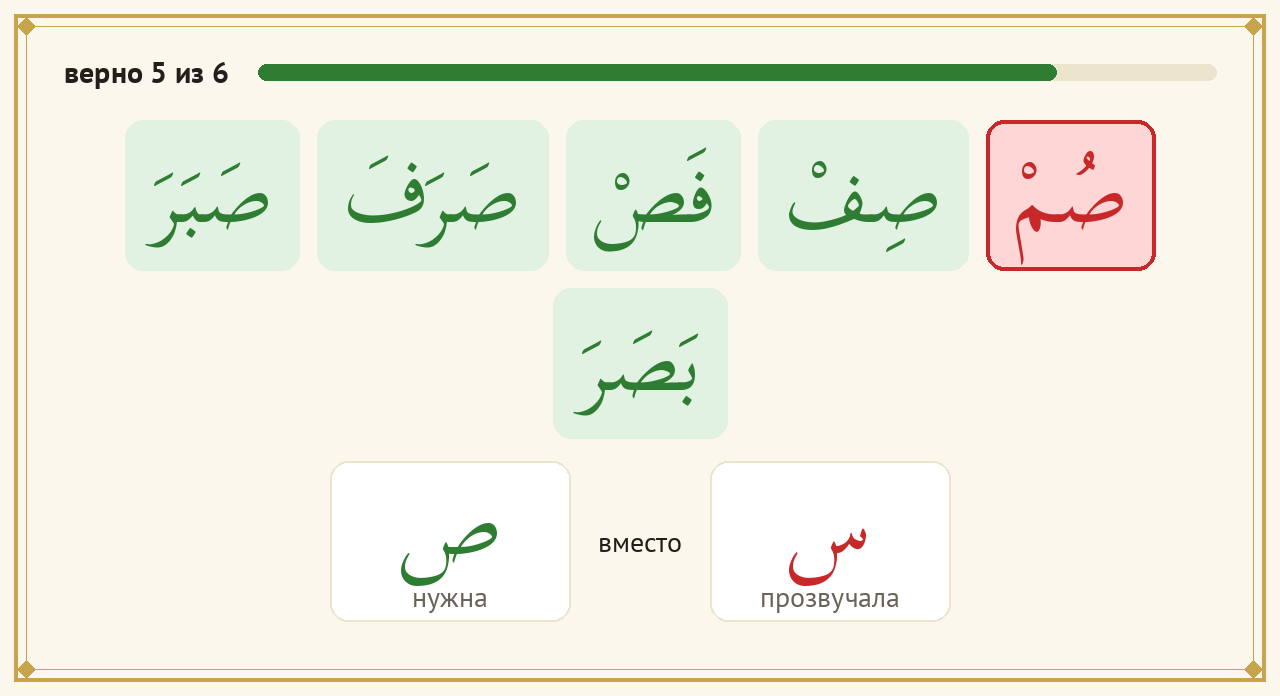
\includegraphics[width=0.78\linewidth]{screen-result.png}
  \caption{After an attempt: the syllable with an error is highlighted in the line.}
\end{subfigure}
\caption{Card images generated by the tutor (interface texts are in Russian).}\label{fig:screens}
\end{figure}

\paragraph{Error review} After an attempt the learner sees the line with the erroneous syllables
highlighted (Figure~\ref{fig:screens}b) and a short review. Each item is a \emph{place}: the syllables
affected by an error, shown as ``how it should sound $\to$ how you said it'' in transcription, with a
half-sentence hint. Clear errors (wrong letter or vowel) come before length errors; at most three places are
listed, the rest are marked on the image; detailed articulation advice is folded under ``more''; and the
review ends with one line: listen to the reference and read the line again. This format follows the feedback
literature reviewed in Section~\ref{sec:lr-capt} and replaced an earlier version that listed every phoneme
and overwhelmed beginners. Praise is given for the task (``this syllable is now correct'') rather than for
the person.

\paragraph{Transcription} A transcription in Russian letters helps a beginner but can become a crutch. As a
compromise between the author's request and teachers' advice, the ``how it reads'' hint on a card is hidden
under a spoiler, so the learner tries the letters first. The transcription follows the scholarly
Krachkovsky system in simplified form: a dot below for emphatic and pharyngeal consonants, a line below for
interdentals, and signs for \emph{'ayn} and hamza, so that \ar{ص} and \ar{س} remain distinct \cite{SRC-051}.

\paragraph{Reference audio} Every card with sound has a ``listen'' button. A teacher's recording, which
teachers can record directly in the bot, takes precedence. Otherwise the tutor uses cuts from the teaching
recitation of al-Husary \cite{SRC-042}; each cut is checked by the model and listed for human review before
use. Speech synthesis was rejected because it does not reproduce tajwid correctly.

\paragraph{Other features} A ``the bot was wrong'' button lets the learner dispute a verdict with a reason;
disputed attempts go first into the annotation queue. Short consolidation questions (``how is this syllable
read?'') revisit learned letters. A streak of days and today's attempts are shown on the home screen. The
first lesson begins with \emph{isti'adha} and \emph{basmala}; the alphabet table on page~10 is shown for
reference without voice checking, because Maksudi teaches sounds, not names.

\section{Research data and annotation}\label{sec:impl-data}

\paragraph{Schema} The attempt is the unit of data. Learners are identified by an internal ID and a pseudonym;
the Telegram ID is stored only in the learner table. Other tables hold the consent log with the version of
the consent text, the entry questionnaire, the curriculum snapshot, detected errors, annotations, annotators
and invitations, learner disputes and an interaction log that records actions without message texts.
Eleven SQL reports and a metrics module compute the GQM measures; development-stub attempts are excluded
everywhere.

\paragraph{Annotation} Annotators work either in Telegram or with an exported package (a CSV file and the
audio). In Telegram, access is limited to a list of annotators or a one-time invitation code valid for a day
and revocable at once; rights are checked on every button press, recordings are sent so that they cannot be
forwarded or saved, and the annotator never sees who the learner is. Imports are strict: one invalid row
rejects the file, repeats add nothing, and a corrected label is added with history. Each label stores the
annotator code, the guide version, its source and the time spent. The error type --- reading, pronunciation or
``unclear'' (Section~\ref{sec:method-s1}) --- is added to the corrected phoneme; the rule with examples from the
book is approved by a human, and the annotation field is a schema change (TD-FN-76).

\paragraph{Metrics and exports} The metrics module computes phoneme-level TA/TR/FA/FR, precision, recall, F1,
diagnosis accuracy, FAR and FRR, Cohen's $\kappa$, Krippendorff's $\alpha$ (tested against the worked example
in Krippendorff's paper \cite{SRC-065}), response-time percentiles, recognition failures and retention.
Datasets are exported only for consenting learners, under pseudonyms, with \texttt{truth.csv} and
\texttt{predictions.csv} in the Iqra'Eval format, so that results can be compared with the shared task
tooling \cite{SRC-066}.

\paragraph{Safety of data} Backups include checksums and are verified; a restore checks hashes, asks for
confirmation and runs in one transaction. A verification command compares the database with the audio store
and finds lost, extra or damaged files and copies that should have been deleted after a withdrawal of
consent.

\section{Training and evaluation pipeline}\label{sec:impl-training}

\begin{notebox}
This section describes the pipeline as designed (technical-debt item TD-FN-72); the code is written in
November--December 2026 and debugged on open data before the pilot. What already exists in version 0.6.0
is stated explicitly.
\end{notebox}

\paragraph{What already exists} Every attempt stores the raw model output with per-phoneme confidence and
attribute probabilities, the canonical variants, the recognised phonemes, the model version and the
SHA-256 of the audio, and annotations store the corrected phonemes. These are the training pairs and the
features for B1: nothing has to be recomputed. The recogniser sits behind a port, and adding a second
recogniser has already shown that a new model plugs in without changing the domain
(Section~\ref{sec:impl-architecture}).

\paragraph{Export and split} An export command assembles the training and test parts from the frozen list
of test learners and writes a datasheet \cite{SRC-123} and fingerprints next to them: of the learner list,
of each part and of the annotation-guide version. Test labels are stored in a directory that a hook forbids
the agent to read; the evaluator loads them itself.

\paragraph{B1} Per-phoneme features are built from the stored model output; training and calibration run on
a CPU. The chosen threshold, the level $\varepsilon$ and the fingerprint of the calibration set are written
into the model version, so every B1 verdict is reproducible.

\paragraph{B2} LoRA fine-tuning runs outside the bot on a GPU (university cluster or cloud, TD-FN-74); only a
small file of adapter weights reaches the bot. B2's model version includes the hash of the base model, of
the adapter and of the training set, so every attempt graded by B2 can be traced to the data the model was
trained on.

\paragraph{Shadow mode and comparison} The second and third recognisers are connected through the same port
in shadow mode: their verdicts are stored next to B0's and are not shown to the learner. Storing shadow
verdicts is a schema change and is approved by a human. The protected evaluator compares the systems on the
test set with one command and writes a report with a passport for the tables in Chapter~\ref{ch:eval}.

\section{Mastery models}\label{sec:impl-mastery}

\begin{notebox}
This section describes a design (technical debt TD-FN-78); the code is written in November--December 2026 and
debugged on simulation and open data before the pilot.
\end{notebox}

\paragraph{Data} The mastery models work on what is already stored: the learner's attempts with time, the book
line, the phoneme-level errors found and the verdict; for test learners, the gold annotation. Through the skill
map each attempt becomes outcomes per skill: a skill of the line is correct if its syllables contain no confirmed
error.

\paragraph{K1 and K2} Bayesian knowledge tracing is implemented as a small pure-Python model in the research
layer: a forward pass over the learner's attempts in time order, parameters per skill, estimation by EM or grid
search on training learners. K2 differs only in its observation model, into which the chosen recogniser's
$\mathrm{FAR}_p$ and $\mathrm{FRR}_p$, computed by the protected evaluator on the training part, are plugged.
Each recogniser (B0, B1, B2) therefore gets its own K2, and the RQ-3 comparison comes down to one call with
different error tables.

\paragraph{Checking before the data} Before the models run on the pilot they are checked on simulated learners
with known parameters: a generator sets the true mastery and the recogniser noise, and the model must recover the
parameters and keep its AUC as the noise grows. The mastery report is produced by the same command as the other
reports, with a passport and a code fingerprint.

\section{Privacy and security}\label{sec:impl-privacy}

\paragraph{Consent and deletion} Learners first see a consent screen; consent to voice recording is separate
and optional, the buttons are not coloured so as not to nudge, and the tutor works without it. Withdrawing
consent deletes recordings and their annotations; ``delete my data'' removes every row and file of the learner.
Logs contain pseudonyms and attempt identifiers but no Telegram IDs, message texts, audio or phonemes; a
filter removes secrets such as the bot token; consent, deletion and annotation events are written only to the
database, not to logs. Tests enforce these rules.

\paragraph{Threat model} A STRIDE analysis covers spoofing (identity only from Telegram-signed user IDs; no
inbound ports thanks to long polling), tampering (audio addressed by SHA-256; restore with verification;
frozen tests against test gaming), information disclosure (pseudonymised exports; agent forbidden to read
learner data and secrets; files with owner-only permissions), denial of service (60-second limit) and
elevation of privilege (parameterised queries, dependency audit, a non-root container, and a hook that blocks
non-existent packages).

\paragraph{Closed pilot and security debt} Some measures --- encryption at rest, a hosting decision, formal
operator status --- depend on institutional decisions. Rather than delay all work, the project runs a closed
pilot and records each postponed measure as a technical-debt item with an explicit trigger: items marked
``before strangers'' must be closed before anyone outside the closed circle is invited.

\section{The development harness}\label{sec:impl-harness}

The tutor was built by one author with Claude Code. The harness around the agent has four layers: context
(instructions, decisions and requirements the agent must know), enforcement (hooks executed by the
environment, not by the model), roles (sub-agents with narrow tasks and limited rights) and the human
(decisions that cannot be delegated). Figure~\ref{fig:harness} shows the loop.

\begin{figure}[ht]
\centering
\resizebox{\linewidth}{!}{% Обвязка ИИ-агента (agent harness): направляющие, датчики, человек (ADR-0011, ADR-0012, ADR-0034, ADR-0039).
% Рамка guides/sensors — SRC-029.
\begin{tikzpicture}[node distance=5mm and 8mm]
  \node[goldbox,text width=3.3cm,xshift=-4mm] (guides) {\textbf{\LANG{Guides}{Направляющие}}\\[-1pt]{\scriptsize CLAUDE.md, ADR, \LANG{skills, requirements}{скиллы, требования}}};
  \node[hot,right=of guides,text width=3.0cm] (agent) {\textbf{\LANG{Coding agent}{ИИ-агент}}\\[-1pt]{\scriptsize\LANG{reason $\to$ act $\to$ observe}{рассуждение $\to$ действие $\to$ наблюдение}}};
  \node[box,right=of agent,text width=3.6cm] (pre) {\textbf{PreToolUse}\\[-1pt]{\scriptsize guard, human\_zones, dep\_check, git\_guard}};
  \node[box,below=of pre,text width=3.6cm] (act) {\LANG{Edit / run}{Правка / команда}\\[-1pt]{\scriptsize\LANG{tests frozen in \texttt{impl}}{тесты заморожены в \texttt{impl}}}};
  \node[box,below=of act,text width=3.6cm] (stop) {\textbf{Stop gate}\\[-1pt]{\scriptsize import-linter, mypy --strict, pytest}};
  \node[box,left=13mm of stop,text width=3.0cm] (rev) {\LANG{Reviewer subagents}{Субагенты-ревьюеры}\\[-1pt]{\scriptsize\LANG{code, architecture, direction}{код, архитектура, направление}}};
  \node[human,left=15mm of rev,text width=3.3cm] (human) {\textbf{\LANG{Human}{Человек}}\\[-1pt]{\scriptsize\LANG{accepts tests, content, commits}{принимает тесты, контент, коммиты}}};
  \node[store,below=8mm of rev,text width=4.2cm,minimum height=1cm] (log) {\LANG{Journals}{Журналы}\\[-1pt]{\scriptsize\LANG{prompts, hook blocks, sessions}{запросы, блокировки, сессии}}};

  \draw[arr] (guides) -- (agent);
  \draw[arr] (agent) -- (pre);
  \draw[arr] (pre) -- node[lab,right]{\LANG{allowed}{разрешено}} (act);
  \draw[arr,draw=lesson] (pre.north) -- ++(0,5mm) -| node[lab,text=lesson,above,pos=0.25]{\LANG{blocked, with reason}{блок с причиной}} (agent.north);
  \draw[arr] (act) -- (stop);
  \draw[arr,draw=lesson] (stop.east) -- ++(5mm,0) |- node[lab,text=lesson,right,pos=0.25]{\LANG{red: keep working}{красно: продолжать}} (act.east);
  \draw[arr] (stop) -- node[lab,above]{\LANG{green}{зелено}} (rev);
  \draw[arr] (rev) -- node[lab,above]{\LANG{STOP $\to$ ask}{СТОП $\to$ вопрос}} (human);
  \draw[arr] (human) -- (guides);
  \draw[darr] (stop.south) |- (log.east);
  \draw[darr] (rev) -- (log);
  \node[lab,above=1mm of guides] {\LANG{feed-forward}{до действия}};
  \node[lab,above=7mm of pre] {\LANG{feedback (sensors)}{после действия (датчики)}};
\end{tikzpicture}
}
\caption{The agent harness: guides, sensors and the human (cf.\ R-06).}\label{fig:harness}
\end{figure}

\paragraph{Hooks} Table~\ref{tab:hooks} lists the eleven hooks. The guard hook fails closed: if it crashes,
the action is refused.

\begin{table}[ht]
\centering\small
\caption{Hooks of the harness.}
\label{tab:hooks}
\begin{tabularx}{\linewidth}{@{}P{3.0cm}P{2.3cm}L@{}}
\toprule
Hook & Event & What it does \\
\midrule
guard & before a tool call & Blocks reading of secrets and learner data, editing tests in the
implementation phase, changing the phase directly, bypassing checks, force pushes; with the training
pipeline (TD-FN-72) it will also block reading test-set labels. \\
human\_zones & before a tool call & Asks for approval with a reason before changes to content, learner
texts, thresholds, reading parameters, schema, dependencies, the checks themselves and the RQ-1
evaluator (with TD-FN-72 and TD-FN-78, also RQ-2 and RQ-3). \\
dep\_check & before a tool call & Blocks packages that do not exist on PyPI; shows version, age,
repository, known vulnerabilities and name similarity for the rest. \\
git\_guard & before a tool call & Forbids forced adds, forbidden paths and secrets in commits; push only
with green checks. \\
format\_python & after a tool call & Formats and lints changed files; returns remaining problems. \\
stub\_notice & after a tool call & Reminds the agent to tell the human when the bot runs with the stub
recogniser. \\
stop\_gate & stop & The agent cannot finish while layer contracts, type checks or tests fail. \\
doc\_sync & stop & ``Changed X --- update Y'': changelog, data dictionary, reports, diagrams, versions of
consent texts, traceability. \\
log\_prompt & prompt & Saves every human prompt with its date (secrets masked). \\
session\_context & session start & Loads the TDD phase, model status, open blocking debt and the last
session summary. \\
notify & notification & Desktop notification when the agent waits for the human. \\
\bottomrule
\end{tabularx}
\end{table}

\paragraph{Test-driven phases} A change goes through explicit phases. In the \emph{tests} phase a test-writer
sub-agent writes failing tests and a test auditor checks that they can catch errors; the author accepts the
tests. In the \emph{implementation} phase tests are frozen by the guard hook and the implementer writes code
until all checks pass. Changing an accepted test requires going back to the tests phase with the author's
consent; the journals record each such case.

\paragraph{Sub-agents} Twenty-one sub-agents have narrow roles. Writers (test writer, implementer, thesis
scribe) may change only their own areas; reviewers (code reviewer, architecture guardian, security auditor,
test auditor, consistency auditor, direction reviewer) have no write access. The direction reviewer checks
whether a change does what the author asked and stays within the agent's authority; when in doubt it must
return STOP with questions for the author rather than a guess. A bot driver walks through the real handlers
in a console mode without Telegram, secrets or the learner database, and a learner simulator reads the
interface as a beginner would, with the caveat that simulated students are not real ones
\cite{SRC-083}.

\paragraph{Decisions and journals} When there is a choice, the agent must present two to four options with
pros and cons instead of choosing silently; the chosen and rejected options are recorded in an ADR. Fifty
ADRs exist, including rejected ideas such as Redis, webhooks, a Mini App and speech synthesis. Each session
ends with a summary of requests, decisions, deviations and unverified items. Commits are prepared by a
dedicated command that runs the checks, audits documentation consistency and asks the author to confirm each
commit and push.

\section{Verification}\label{sec:impl-verification}

The test suite runs in under a minute without the model or the network and currently has 736 passing tests.
It combines unit tests of the domain, integration tests of repositories on SQLite (and PostgreSQL in CI),
end-to-end tests of the bot flow through the dispatcher, architecture tests (layer contracts, migrations
match the schema, every use case is registered, logs contain no forbidden fields, documents link to existing
files) and property-based tests that must hold for any reference and any model output: reading exactly the
reference gives a perfect result; the score stays within 0--100 and every error points into the reference;
the assessment is deterministic; ``excellent'' is given only without errors; an unread tail points to an
existing syllable; and the best reference is the closest one, the first on ties \cite{SRC-096}. The suite
runs 300 random cases per property; a one-off run with 5\,000 cases per property found no violation. Line coverage is above
97\,\% with a CI minimum of 80\,\%; mypy runs in strict mode. Continuous integration adds secret scanning,
dependency vulnerability audit, declared-dependency checks, a static check of the workflows themselves and a
Docker build. An automated traceability report shows that 59 of 60 traced requirements are covered by passing
tests.
